\chapter{Solicitar OS - Cancelamento}

\section{Contextualização}

De acordo com as EPEs e os Protótipos que temos até o momento, o processo de \textbf{Solicitar Ordem de Serviço} está bem documentado e pode ser resumido assim:

\begin{enumerate}
	\item Solicitante acessa a tela ``Solicitar Ordem de Serviço'';
	\item Clica em ``Novo'';
	\item Preenche um formulário com as informações da ``Nova Solicitação'' inserindo anexos e etc;
	\item Clica em ``Enviar para Assinatura'';
	\item O Sistema cria no SEI o Processo contendo o documento do tipo “SOLICITAÇÃO DE SERVIÇO DA ASSESSORIA LEGISLATIVA” já preenchido com as informações fornecidas pelo Solicitante no Sistema ASSEL.
	\item \textbf{Aqui o Status da Solicitação é ``Enviado para Assinatura''.}
	\item Aguarda Assinatura.
	\item Após assinatura, o Status da Solicitação passa a ser ``Em Execução''.
	\item Em seguida, o Sistema cria a solicitação e envia para a ``Caixa de Entrada'' da ASSEL e assim o processo de elaboração da Solicitação começa seguindo o modelo BPMN definido.
\end{enumerate}

\section{Objetivo}

	O Dashboard do Solicitante mostra as Solicitações com seus respectivos Status permitindo-se ``Visualizar'' ou ``Cancelar''.

	\begin{figure}[htbp!]
	\centering
	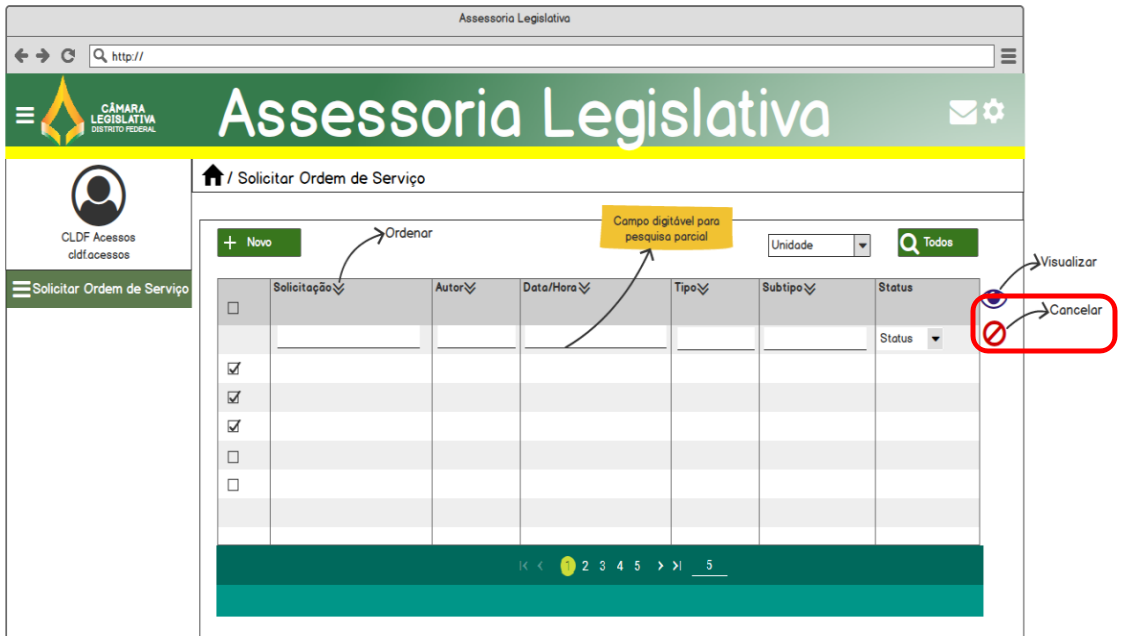
\includegraphics[width=0.9\textwidth]{fig/solicitaros-sei/assel-solicitaros-cancelar.png}
	\end{figure}
	
	O objetivo desse documento é orientar como o processo de Cancelamento deve ocorrer no SEI.
	
\section{Estados Possíveis}	

De acordo com a EPE ``Solicitar Ordem de Serviço'' funcionalidade 04 ``Cancelar'', podem existir os seguintes estados de uma Solicitação:

\begin{itemize}
	\item \textbf{Enviado para Assinatura}: Solicitação não assinada aguarda assinatura para entrar em execução.

	\item \textbf{Em Execução}: Solicitação assinada entrou em execução.

	\item \textbf{Pendência}: Solicitação assinada está em execução mas apresenta pendência que deve ser resolvida pelo Solicitante para continuar.

	\item \textbf{Concluído}: Solicitação assinada foi concluída com sucesso.
	
	\item \textbf{Descontinuado}: Solicitação assinada foi cancelada (tanto pelo Solicitante quanto por outro Ator).
	
	\item \textbf{Cancelado}: Solicitação não assinada foi cancelada.
	
	
\end{itemize}

Dessas, apenas os seguintes estados podem ser cancelados:
\begin{itemize}
	\item Em Execução: Uma solicitação em execução, após ser cancelada, passa a ter o estado de ``descontinuado''.
	\item Enviado para Assinatura: Uma solicitação enviada para assinatura, após ser cancelada, passa a ter o estado de ``cancelada''.
\end{itemize}

É importante ressaltar:


Uma \textbf{Solicitação ``Em Execução'' ou ``Pendência''}  podem ser canceladas  mediante um Termo de Cancelamento assinado no SEI.

Uma \textbf{Solicitação ``Enviada para Assinatura''} e, portanto, não assinada, pode ser cancelada sem depender de um Termo de Cancelamento assinado no SEI.

Então existem dois casos possíveis de cancelamento:

\begin{itemize}
	\item Solicitação por parte do Solicitante de Cancelamento de Solicitações em Execução/Pendência;
	\item Solicitação por parte do Solicitante de Cancelamento de Solicitações Enviadas para Assinatura;
\end{itemize}


\section{Cancelamento de Solicitações em Execução ou Pendência}	

Conforme dito, uma Solicitação ``Em Execução'' pode ser cancelada mediante um Termo de Cancelamento assinado no SEI.

Já que o início da execução de uma solicitação depende de um instrumento que é a assinatura de um documento de solicitação no SEI, a sua interrupção e extinção antes de ser concluída também vai depender da assinatura de um documento no SEI. 

Esse documento é o \textbf{Termo de Cancelamento}.   

Assim, vamos ao passo-a-passo de como deveria se dar o cancelamento de uma \textbf{Solicitação Em Execução}.


\large
\begin{center}
	\textbf{Cancelamento de Solicitações em Execução / Pendência - Início}
\end{center}
\normalsize


\subsection{Solicitante escolhe a Solicitação em Execução e manda Cancelar}	

Solicitante vai no dashboard, escolhe a solicitação e clica em ``Cancelar''. Neste momento, conforme EPE e Protótipos, abre-se uma janela pedindo que o usuário digite uma justificativa e confirme o pedido de cancelamento clicando em ``Enviar para a ASSEL''.

\subsection{Sistema ASSEL reabre o processo relacionado a essa OS na Unidade do Solicitante}

A Solicitação possui um atributo para guardar o número do processo do tipo \textbf{``Assessoria Legislativa: Consulta, estudo, parecer, discurso e proposições legislativas''} que foi criado na Unidade do Solicitante no SEI e contém o documento com a Solicitação de Abertura de OS, que foi assinada e enviado para a ASSEL (e concluído lá).

Então o Sistema da ASSEL deve ir na Unidade do SEI do Solicitante e reabrir esse processo.

\begin{exemplo}[1]{Descobre}
	Sistema ASSEL descobre que o processo do SEI relacionada à Solicitação que deve ser cancelada é a de número 00001-00000001/2021-01.
\end{exemplo}

\begin{exemplo}[1]{Reabre}
	Daí o Sistema ASSEL vai na Unidade do Solicitante no SEI e reabre esse processo lá.
\end{exemplo}


\subsection{Sistema ASSEL gera o Termo de Cancelamento}

Dentro do processo do SEI (reaberto na Unidade do Solicitante) deve ser gerado o documento do tipo \textbf{``TERMO DE CANCELAMENTO''} usando o modelo repassado com as seguintes informações automaticamente preenchidas pelo Sistema ASSEL:

\subsubsection{SOLICITANTE}

Deputado/órgão: \textbf{Preencher de acordo com a OS}

Contato:  \textbf{Preencher de acordo com a OS}

Ramal:  \textbf{Preencher de acordo com a OS}

\subsubsection{PEDIDO DE CANCELAMENTO}

Solicito o cancelamento da Ordem de Serviço Nº XXXXXXX. Compreendo que a execução do
serviço será interrompida e essa é uma operação irreversível.

\subsubsection{JUSTIFICATIVA}

Deve estar escrito a mesma justificativa que foi escrita pelo Solicitante na caixa de texto. 

\subsection{Sistema ASSEL cria, caso necessário, o Bloco de Assinatura}	


\subsubsection{Caso o Usuário Solicitante que pediu o cancelamento pertença à Unidade Solicitante do SEI}

Se a Unidade Solicitante possui o Usuário que está fazendo a Solicitação de Cancelamento como um usuário pertencente a ela\footnote{Isso deve ser verificado usando a API do SEI}, não precisa criar Bloco de Assinatura. E nem seria possível fazer isso. 

Nesse caso, sistema deve avisar ao Usuário para assinar o documento especifico do processo especifico da unidade determinada conforme exemplo de mensagem abaixo:


\begin{exemplo}[1]{Exemplo de Mensagem em Caso de Não Haver Bloco de Assinatura}
	Por favor, assinar o documento SEI Nº 0000002 do processo 00001-00000001/2021-01 na Unidade ``NOME DA UNIDADE'' para efetivar o cancelamento. 
	
	\vphantom{espaço vertical em branco}			
	
	Após assinatura, o Sistema ASSEL se encarregará de tramitar o processo para a Assessoria Legislativa.
	
	\vphantom{espaço vertical em branco}					
	
	\framebox[3cm][c]{OK}
\end{exemplo}



\subsubsection{Caso o Usuário Solicitante NÃO Pertença à Unidade Solicitante do SEI}


\begin{enumerate}
	
	
	\item  Se a Unidade Solicitante não possui o Usuário que está fazendo a Solicitação, então será mostrado uma janela \textbf{Popup} contendo um \emph{combobox} listando todas as unidades (exceto a Unidade Solicitante\footnote{Lembrar  que na lista de unidades do combobox não deve constar a Unidade do SEI onde está sendo criado o Bloco de Assinatura já que não é possível criar um Bloco de Assinatura e disponibiliza-lo para a mesma unidade de origem.}) de forma que o Usuário possa escolher para qual Unidade do SEI deverá ser disponibilizado o Bloco de Assinatura que será assinado.
	
	\begin{env-popup}[1]{Exemplo de Popup}
		Por favor, escolha a unidade do SEI onde você deseja assinar o cancelamento:
		
		\vphantom{espaço vertical em branco}			
		
		\framebox[8cm][c]{CMI}		
		\framebox[0.5cm][c]{$\nabla$}
		
		\vphantom{espaço vertical em branco}					
		
		
		\framebox[3cm][c]{OK}
		\framebox[3cm][c]{CANCELAR}
		
	\end{env-popup}	
	
	\item Quando o usuário escolhe uma Unidade do SEI e clica em OK, o sistema verifica se o Usuário tem acesso no SEI àquela unidade \emph{e se possui capacidade de assinar documentos nela}. Se sim, prossegue. Se não, pede que ele escolha uma Unidade onde ele tem acesso e pode assinar. Só prossegue quando o Usuário escolher uma unidade que atenda esses dois requisitos. 	
	
	
	\item Quando finalmente o usuário escolhe uma unidade na qual ele tem acesso e tem permissão de assinar documentos, então o sistema cria o bloco de assinatura na Unidade Solicitante.
	
	\item O Bloco de Assinatura deve ser criado com a seguinte ``Descrição'' padrão:
	
	\begin{exemplo}[1]{Descrição do Bloco de Assinatura}
		Sistema ASSEL - Cancelamento de Ordem de Serviço
		
		Unidade Solicitante: Gabinete do Deputado Fulano
		
		Usuário Solicitante: Nome Completo do Usuário Solicitante do Cancelamento
	\end{exemplo}
	
	\item No campo ``Unidades para Disponibilização'' deve ser escolhido a unidade escolhida pelo Usuário Solicitante no \textbf{Popup}.
	
	\begin{figure}[htbp!]
		\centering
		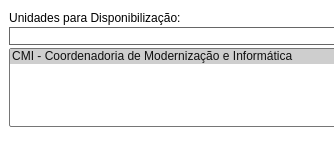
\includegraphics[width=0.8\textwidth]{fig/solicitaros-sei/ex3.png}
		\caption{Exemplo de Unidade para Disponibilização do Bloco de Assinatura}
		\label{fig:solitaros-sei:ex3}
	\end{figure}
	
	
	\item Em seguida, o sistema cria o Bloco de Assinatura dentro da Unidade Solicitante  e incluí nele o \textbf{Termo de Cancelamento} do processo relativo à OS que precisa ser assinado. Finalmente, o sistema disponibiliza o Bloco de Assinatura para ser assinado pelo Usuário Solicitante.
	
	\item O número do bloco de assinatura para cancelamento deve ser armazenado como atributo da Solicitação no sistema ASSEL. \footnote{O número do Bloco de Assinatura novo criado para assinar o Termo de Cancelamento pode ser armazenado no lugar do Bloco de Assinatura antigo (usado na primeira vez para assinar a Solicitação). Não tem problema, se for o caso, revisamos isso depois.}
	

	
	\item De forma semelhante, o Sistema ASSEL mostra a mensagem ao usuário informando que ele deve assinar o documento no Bloco de Assinatura criado.
	
	\begin{exemplo}[1]{Exemplo de Mensagem em Caso de Haver Bloco de Assinatura}
		Por favor, assinar o documento SEI Nº 0000002 do processo 00001-00000001/2021-01 disponível no Bloco de Assinatura Nº 00002 disponibilizado para a Unidade UNIDADE-ESCOLHIDA. 
		
		\vphantom{espaço vertical em branco}			
		
		Após assinatura, o Sistema ASSEL se encarregará de tramitar o processo para a Assessoria Legislativa efetivando o cancelamento.
		
		\vphantom{espaço vertical em branco}	
		
		\framebox[3cm][c]{OK}
	\end{exemplo}	
	
	
\end{enumerate}	


\subsection{Sistema ASSEL aguarda a assinatura do Termo de Cancelamento}


A partir daí o sistema passa a monitorar o Termo de Cancelamento do SEI esperando que ele seja assinado.

Importante notar que o cancelamento da Solicitação no sistema só vai ser efetivado após o Sistema ASSEL detectar que o ``Termo de Cancelamento'' gerado foi assinado.

\subsection{Termo de Cancelamento é assinado pelo Solicitante}

Usuário acessa o SEI e assina o documento.

Quando o Termo de Cancelamento é assinado pelo Solicitante, então o seu estado no dashboard do Solicitante dentro do sistema ASSEL passa a ser ``DESCONTINUADO''. E aí o sistema faz o que tiver que ser feito para cancelar a solicitação\footnote{Essas coisas que o Sistema fará ainda não foram levantadas completamente e dependerá de novas reuniões de levantamento de requisitos}.

\subsection{Sistema ASSEL cancela a disponibilização e conclui o Bloco de Assinatura caso ele exista}

Após assinatura, se foi criado Bloco de Assinatura, o Sistema cancela a disponibilização do Bloco de Assinatura para as unidades e o conclui.

\subsection{Sistema Envia Processo para a Unidade ASSEL}

O Sistema envia o processo para a Unidade ``ASSEL''.

\subsection{Sistema Recebe o Processo na Unidade ASSEL}

Do lado da ASSEL, o próprio sistema recebe o processo.

\subsection{Sistema atribui ao processo um Acompanhamento Especial}

Sistema marca o processo com o Acompanhamento Especial especificado.

\subsection{Sistema conclui o processo}

Sistema conclui o processo para remove-lo da lista de ``Recebidos'' do SEI da Unidade ASSEL.


\subsection{A solicitação passa a ter o estado de ``Descontinuado''}

\Large
\begin{center}
	\textbf{Cancelamento de Solicitações em Execução / Pendência - Final}
\end{center}
\normalsize

\section{Cancelamento de Solicitações Enviadas para Assinatura}	

Trata do cancelamento de solicitações enviados para assinatura, mas que ainda não foram assinadas.

É mais fácil porque a Solicitação, por não ter sido assinada no SEI, ainda não começou o efetivo trâmite dentro da ASSEL.

\subsubsection{Resumo do que aconteceu até agora:}

\begin{enumerate}
	\item Usuário preencheu o formulário de Solicitação e enviou para a ASSEL;

	\item Sistema ASSEL criou novo processo no SEI;
	
	\item Sistema ASSEL criou documento da OS no processo do SEI;
	
	\item Sistema ASSEL inseriu os anexos no processo;
	
	\item Sistema ASSEL criou, caso necessário, o Bloco de Assinatura;
	
	\item Sistema ASSEL \textbf{ainda} aguarda assinatura do Usuário Solicitante;
\end{enumerate}
  
\large
\begin{center}
	\textbf{NO ENTANTO}
\end{center}
\normalsize

\begin{enumerate}
	\item Solicitante desistiu da Solicitação, mas ainda não assinou a Solicitação.
	
	\item Solicitante resolveu ``Cancelar'' a Solicitação de estado ``Enviados para Assinatura''.	
\end{enumerate}


Portanto vamos detalhar o passo-a-passo do que deveria ocorrer nesse caso:

\Large
\begin{center}
	\textbf{Cancelamento de Solicitação enviadas para Assinatura - Início}
\end{center}
\normalsize


\subsection{Sistema ASSEL cancela e conclui Bloco de Assinatura caso ele exista}

Se foi criado Bloco de Assinatura, o Sistema cancela a disponibilização do Bloco de Assinatura para as unidades e o conclui.

\subsection{Sistema ASSEL exclui todos os anexos da solicitação inseridos no processo}

Todos os anexos automaticamente criados pelo sistema ASSEL são excluídos. 

\subsection{Sistema ASSEL exclui a minuta da OS da Solicitação}

A Minuta do Formulário da Ordem de Serviço que deveria ser assinada é excluída.

\subsection{Sistema ASSEL conclui o processo na Unidade Solicitante}

O próprio Sistema ASSEL conclui o processo na Unidade Solicitante.

\subsection{O estado da Solicitação dentro do Sistema ASSEL passa a ser ``Cancelado''}

\Large
\begin{center}
	\textbf{Cancelamento de Solicitação enviadas para Assinatura - Final}
\end{center}
\normalsize